The tool that allows us to easily manage bibliography is called BiBTeX. In particular, we are using a \emph{package} called \verb|natbib| that gives us some extra features.
Using it has two distinct moments: Adding an entry to our bibliography, and citing.

\clearpage
\subsection{Creating a bibiliography}
A bibliography file has a \verb|.bib| extension, and each entry has a very specific format.
Let's start with creating the file \verb|bibliography.bib|, so our working directory looks like this:
\begin{verbatim}
Example
├── bibliography.bib
└── example.tex
\end{verbatim}

Each entry has a source, whether \verb|article|, \verb|book|, \verb|misc| or many more and has the following format:
\begin{lstlisting}
@article{ GerberLeahR2005, %Unique identifier
  author    = {Gerber, Leah R and Beger, Maria and McCarthy, Michael A and Possingham, Hugh P},
  title     = {A theory for optimal monitoring of marine reserves},
  issn      = {1461-023X},
  journal   = {Ecology letters},
  pages     = {829--837},
  volume    = {8},
  publisher = {Blackwell Science Ltd},
  number    = {8},
  year      = {2005},
  edition   = {Editor, Ransom Myers Manuscript received 15 March 2005 First decision made 21 April 2005 Manuscript accepted 6 May 2005},
},
\end{lstlisting}

It's worth highlighting that the basic format is essentially \verb|@article{ID,...}|, with each entry being separated by commas.
BiBTeX will handle ``et al'' and other conventions as long as you stick to the following format:
\begin{lstlisting}
author = {LastName1, FirstName1 and LastName2, FirstName2 and...}
\end{lstlisting}

The good side is that you rarely, if ever, need to type it out yourself.
When you find an article through UCL's library, JAMA, Science Direct and many other resources, there will be an option to \textbf{export citation to BiBTeX}.
Simply copy the contents to your bibliography file and you're ready to cite!

\subsection{Manually adding a bibliography entry}
While using VSCode, you can scaffold a bibliography entry in a \verb|.bib| file.
Simply type \verb|@| and press \verb|Ctrl+space|, and it will generate the skeleton for an entry.
Generally this is only used for citing random websites, so you will want to pick the \verb|@misc| option.

\subsection{Citations}
Now we just need to let our document know where to find our bibliography file and we can use \verb|\cite{}| to include citations.
Every entry that that is cited, automatically gets added to a Reference section at the end of your document.
\lstinputlisting[language=tex, caption={example.tex}]{"Example/example.tex"}

Giving us the following output:
\begin{figure}[h]
  \centering
    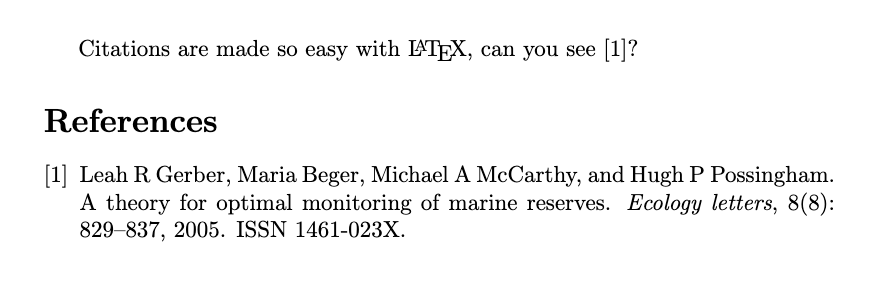
\includegraphics[]{figures/references.png}
  \label{fig:references}
\end{figure}

\verb|\usepackage[square,numbers]{natbib}| is what determines that in-text citations is \textbf{[1]}.
Alternatively if you prefer \textbf{(Gerber et al, 2005)}, use \verb|\usepackage[round]{natbib}|, and \verb|\citep{}| instead of \texttt{\textbackslash cite\{\}}:
\begin{lstlisting}
\usepackage[round]{natbib}
...
\citep{GerberLeahR2005}
\end{lstlisting}

The \verb|natbib| package gives us the \verb|bibliographystyle{unsrtnat}| option, which determines the style of the references.
There are others, as well as more information on \verb|natbib|, which you can find more about on \href{https://ftp.eq.uc.pt/software/TeX/macros/latex/contrib/natbib/natnotes.pdf}{this} link. 

A really important feature is that the editor even suggests the authors we have added to our \verb|.bib| file.
\begin{figure}[h]
  \centering
  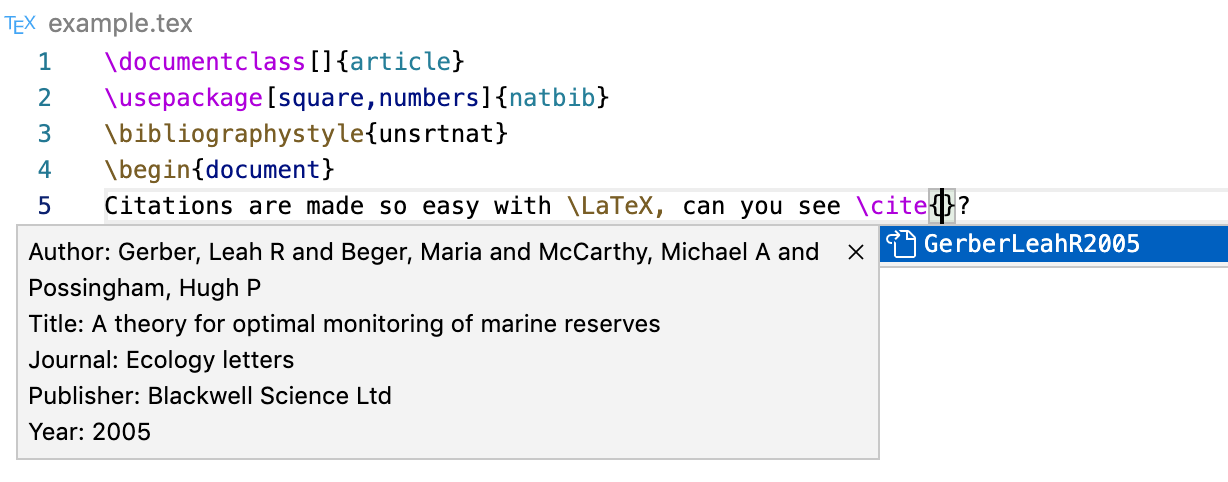
\includegraphics[width=\textwidth]{figures/intellisense.png}
  \caption{Autocomplete from our bibliography file}
  \label{fig:intellisense}
\end{figure}

Automatically generating numbers for figures, tables and correcting any citations is a key feature of \LaTeX.
This means we can easily refer to a figure, move it around and it will correctly choose its number.
Before we get into adding all that it is a great idea to take a detour and discuss organisation.